\documentclass[12pt]{article}

\usepackage{amsmath, amssymb, amsthm, graphicx, fancyhdr, textcomp, enumerate, diagbox, tcolorbox, esvect, tikz, adjustbox}


\graphicspath{{./images/}}


\usepackage{halloweenmath, tikzsymbols}

\newcommand{\R}{\mathbb{R}}
\newcommand{\Z}{\mathbb{Z}}
\newcommand{\C}{\mathbb{C}}
\newcommand{\N}{\mathbb{N}}
\newcommand{\Q}{\mathbb{Q}}
\newcommand{\Arg}{\mbox{Arg}}
\newcommand{\Log}{\mbox{Log}}


%geometry/topology
\newcommand{\bndry}{\partial}


\newcommand{\infsum}{\sum_{n = 1}^{\infty}}
\newcommand{\pf}{\fbox{proof}}
\newcommand{\cor}{\fbox{corollary}}

\theoremstyle{definition}

\newtheorem*{definition}{Definition}
\newtheorem{lemma}{Lemma}
\newtheorem{theorem}{Theorem}
\newtheorem{corollary}{Corollary}
\newtheorem{proposition}{Proposition}
\newtheorem{remark}{Remark}
\newtheorem{conjecture}{Conjecture}
\newtheorem{example}{Example}
\newtheorem{problem}{Problem}


\title{Modern Geometry}
\author{August}

\begin{document}

\maketitle

\begin{lemma}
In a tetrahedron, every vertex $v$ is adjacent to three of the four triangular faces. Moreover, each of these triangular faces share exactly two vertices, one of which is $v$.
\end{lemma}
\begin{proof}
This can be verified simply by noting that the polyhedron is essentially symmetric (at least in terms of what's adjacent to what), so we need only consider one vertex without losing generality. Consider the vertex $A$ as shown in the image.\\

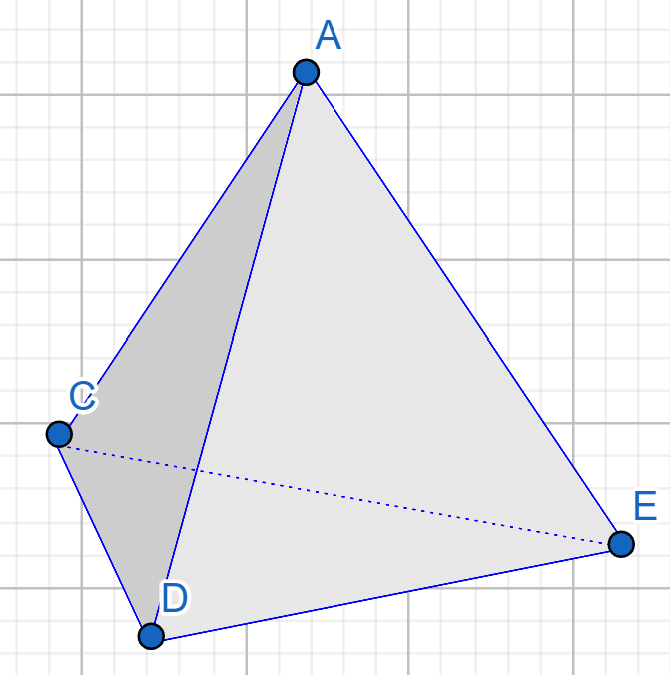
\includegraphics[scale=0.5]{tetrahedron.png}\\

In this image, $A$ is adjacent to the triangles $ACD$, $ADE$, and $ACE$. Each of these triangles share at least two vertices, one of which is $A$. 
\end{proof}


\begin{lemma}
No diagonals of the Schonhardt polyhedron can be drawn. 
\end{lemma}
\begin{proof}
Every face of the Schonhardt polyhedron is a triangle, as is clear from it's construction. As a result, if a diagonal were to be drawn, that triangle would have to be a body diagonal. But this is impossible, for upon un-rotating the top triangle so that the diagonal edges on the quadrilateral faces lie flat against the surface, we would have a body diagonal for the rectangular prism. The rectangular prism has no body diagonals. This is apparent if we simply draw all possible diagonals. Hence no diagonals can be drawn. \\

Alternatively, we can deduce this by looking at the top view. Other than the existing edges, the only possible remaining ones are $AR$ (which is covered by the annoying letter "D"), $CQ$, and $PB$. The fact that these are the only possible ones comes from the fact that, other than these other line segments, we actually have a complete graph on the vertices from the existing edges! (As I'm sure the reader would like) As shown in the figure, each of segments leaves the interior of the polyhedron. So no diagonals can be drawn.


 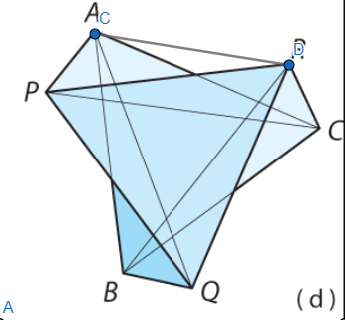
\includegraphics[scale=1]{attempteddiagonal.png} 
\end{proof}

\begin{proposition}
The Schonhardt polyhedron cannot be tetrahedralized.
\end{proposition}

\begin{proof}
In any tetrahedralization, all vertices must be part of a tetrahedron. Let us chose the vertex $Q$ shown in the image. For it to be a vertex of some tetrahedron in some tetrahedralization, it must be the case that $Q$ is adjacent to three triangles of one tetrahedron. Because no body diagonals can be drawn, these triangles must exist on the face. Notice that $Q$ is adjacent to four triangles : $PQA$, $PQR$, $QAB$, $RQB$. Removing any one of these four, the two triangles adjacent to the one removed do not share two vertices with each other. Hence $Q$ cannot be part of a tetrahedron. Thus the Schonhardt polyhedron cannot be tetrahedralized.\\


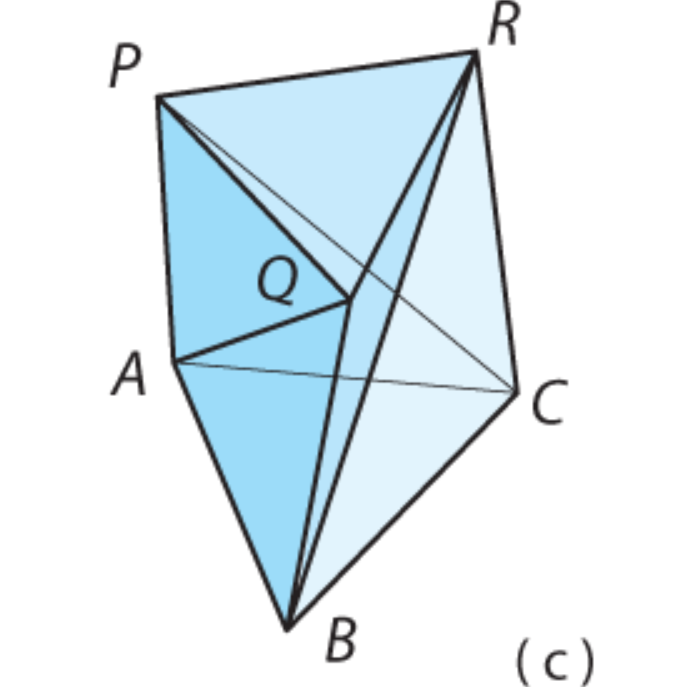
\includegraphics[scale=0.5]{schoonhardt.png} 

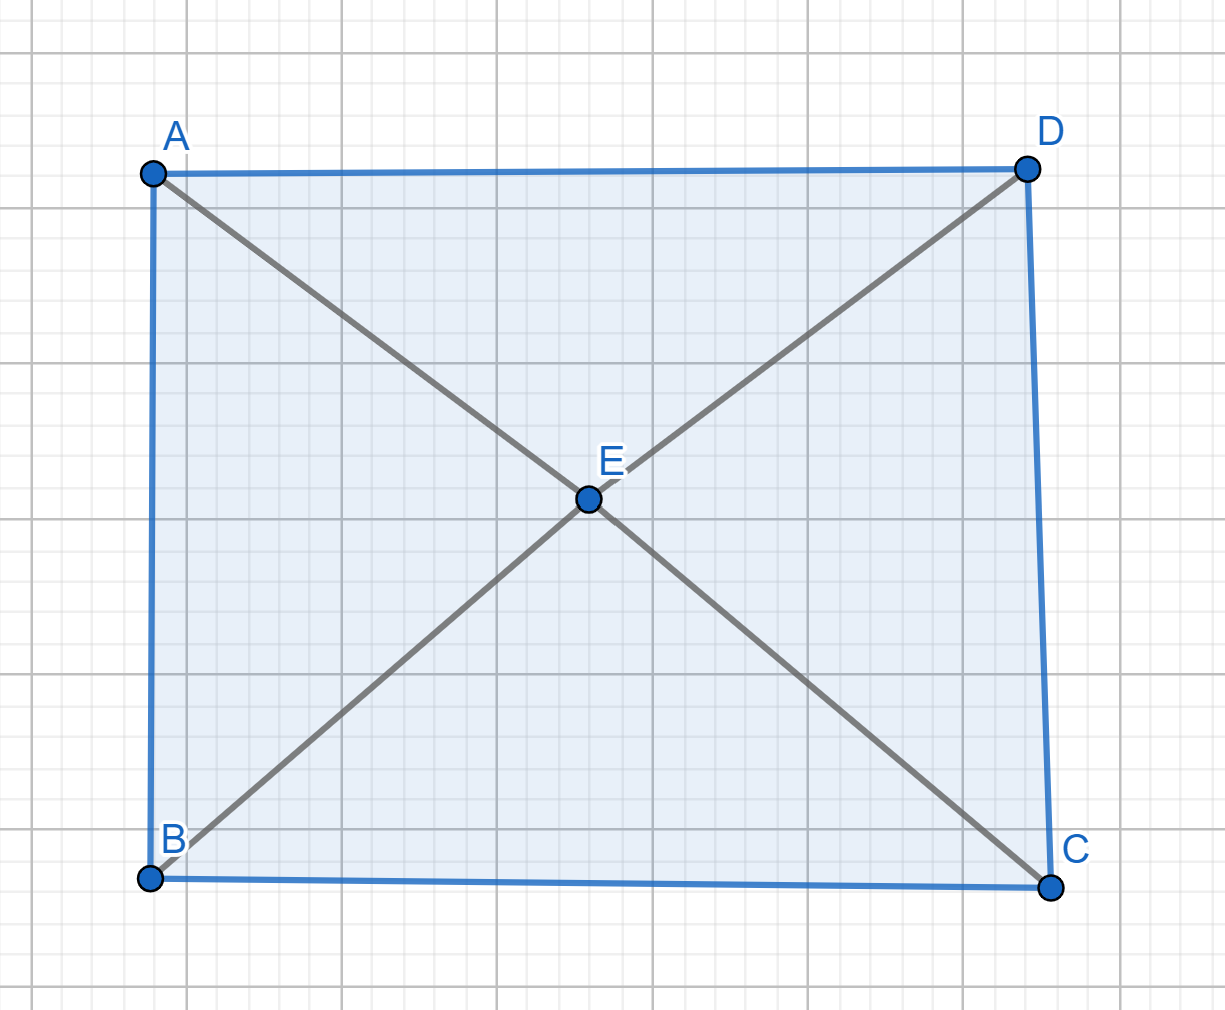
\includegraphics[scale=0.5]{four_triangles.png} 
Note that in this image, the vertex $Q$ corresponds to $E$, $P$ to $A$, $R$ to $D$, $B$ to $C$, and $A$ to $B$. I don't yet know how to rename vertices in geogebra lol! 
\end{proof}

\begin{lemma}
Any triangle is covered by a guard placed at any of its vertices.
\end{lemma}
\begin{proof}
I take this as obvious. Since we don't have formal axioms, I probably have to use meaning where form won't do the trick.
\end{proof}

\begin{proposition}
All quadrilaterals can be covered with a single guard.
\end{proposition}

\begin{proof}
 Let $P$ be a quadrilateral. Since every polygon can be triangulated, $P$ can be triangulated. Moreover, by Theorem  this triangulation has $4-2 = 2$ triangles. Each triangle has three vertices. There are only four vertices of $P$ to go around. Therefore these two triangles must share a vertex $v$ (I think this is the pigeonhole principle). Moreover, this vertex covers both of these triangles, as follows by the lemma. Because the union of these triangles is the entire polygon $P$, it follows that a guard placed at $v$ covers all of $P$.
\end{proof}

\begin{proposition}
Every pentagon can be covered with a single guard.
\end{proposition}

\begin{proposition}
From Corollary 1.9 of the textbook, there exists at least one ear for any triangulation (and there is a triangulation). Removing this ear gives us a quadrilateral. Now triangulate the remaining quadrilateral. Because the quadrilateral has four vertices, any triangulation of it has $4-3 = 1$ diagonals, $d$. Hence all of the triangles in any triangulation share that one edge. Now chose any edge $e_1$, and a vertex on it $v_1$ connected to the diagonal $d$. This vertex must connect to a non-adjacent vertex, and this must skip one edge $e_2$ on both sides. Notice $e_1$ is adjacent to one other edges $e_3$ which shares the vertex $v_1$, and this cannot be $e_2$ for it is not adjacent. Notice also that $e_2$ is adjacent to one edge $e_4$ which shares the vertex connecting to $d$. Since $e_1$ is not adjacent to $e_2$, $e_4$ is not $e_1$. Similarly, if $e_3 = e_4$, then we would have a diagonal connecting an edge to itself, which is nonsense! Hence $e_3 \ne e_4$. So we have four distinct edges of the quadrilateral $Q$, all of which share a vertex with $d$. So $d$ must also share a vertex with the edge containing the ear. Chose this vertex. This vertex is part of each triangle in this triangulation of the entire pentagon. Hence it covers each of these triangles, thereby covering the entire pentagon. 
\end{proposition}

\begin{remark}
The most interesting number is $5$. It is the greatest and least element in the size of many sets. It is the breaking point, and the starting point, of so many interesting things. It is the smallest degree of polynomails for which a general formula in terms of extracting roots, multpilying, and adding, does not exist; and all polynomials of higher degree than $5$ have no general formula for their roots. It is the smallest number of elements so that the symmetric group on those elements is not solvable. It is also the smallest number of vertices for which a regular polygon can be stellated. It is also, as we have just shown, the largest number of vertices that forces a polygon to be coverable by a single guard. It is also prime, which is nice.
\end{remark}

\begin{example}
Consider the polygon shown below, with guards placed at the points $A$, $B$, $E$ and $F$. All of it's boundary is covered, but it is not covered.
\end{example}
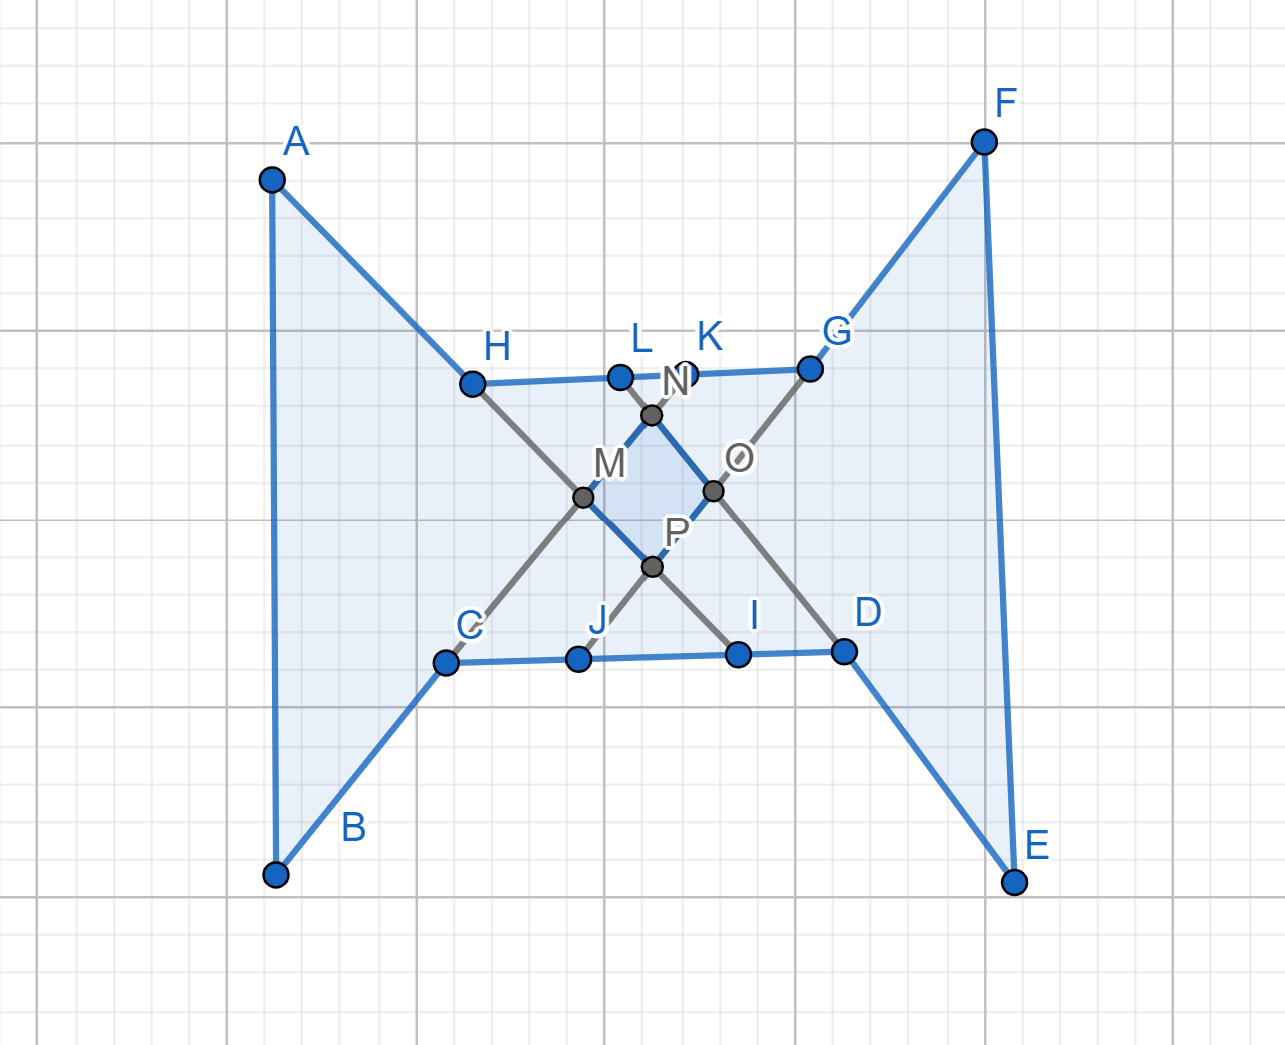
\includegraphics[scale=0.5]{boundary.png}\\

In fact, this is not just an example, but a method for constructing one. We start with a rhombus, $OPMN$, and extend two pairs of adjacent edges outward in the opposite direction of where they meet. Beyond where these rays extend past the boarder of the rhombus, connect these points on both sides to create the edges $HG$ and $GD$. Now extend further past this, ending at points $A$, $F$, $E$, and $B$. Finally, draw the edges $AB$, $FE$. Place guards at the vertices $A$, $B$, $F$, $E$. As can be seen, $A$ covers all of the region $AICB$, and similarly for all the vertices, but is blocked by the boarder of the "inner part" of the polygon. The "lines of sight" meet up so that they intersect, all the while leaving the center rhombus uncovered.


\begin{definition}
Let $P$ be a polygon, and let $x$ be a point in $P$. A point $y$ in $P$ is \textbf{2-visible} by $x$ if the line segment $xy$ crosses the boundary of $P$ at most twice. Let $T(x,y)$ be the proposition $y$ "$y$ is 2-visible by $x$". The \textbf{2-kernel} of $P$ is the set $ S = \{x\in S: \forall y\in P, T(x,y)\}$.
\end{definition}

\begin{definition} (based on complex analysis)
S region $S$ is connected if for all $x,y\in S$ there exists a polygonal path $\Pi$ connecting the two points. Let's say that a \textbf{polygonal path} $\Pi$ is defined to be a finite collection of vertices $v_1,\dots,v_n$ and edges $v_1v_2, \dots, v_{n-1}v_n$. The $i$th vertex of $\Pi$ is denoted $ \Pi[i] = v_i$. We could say that $x$ and $y$ are connected if there exists a point polygonal path $\Pi$ such that $\Pi[1] = x $ and $\Pi[2] = y$. 
\end{definition}

\begin{proposition}
There exists a polygon $P$ such that the 2-kernel of $P$ is disconnected.
\end{proposition}
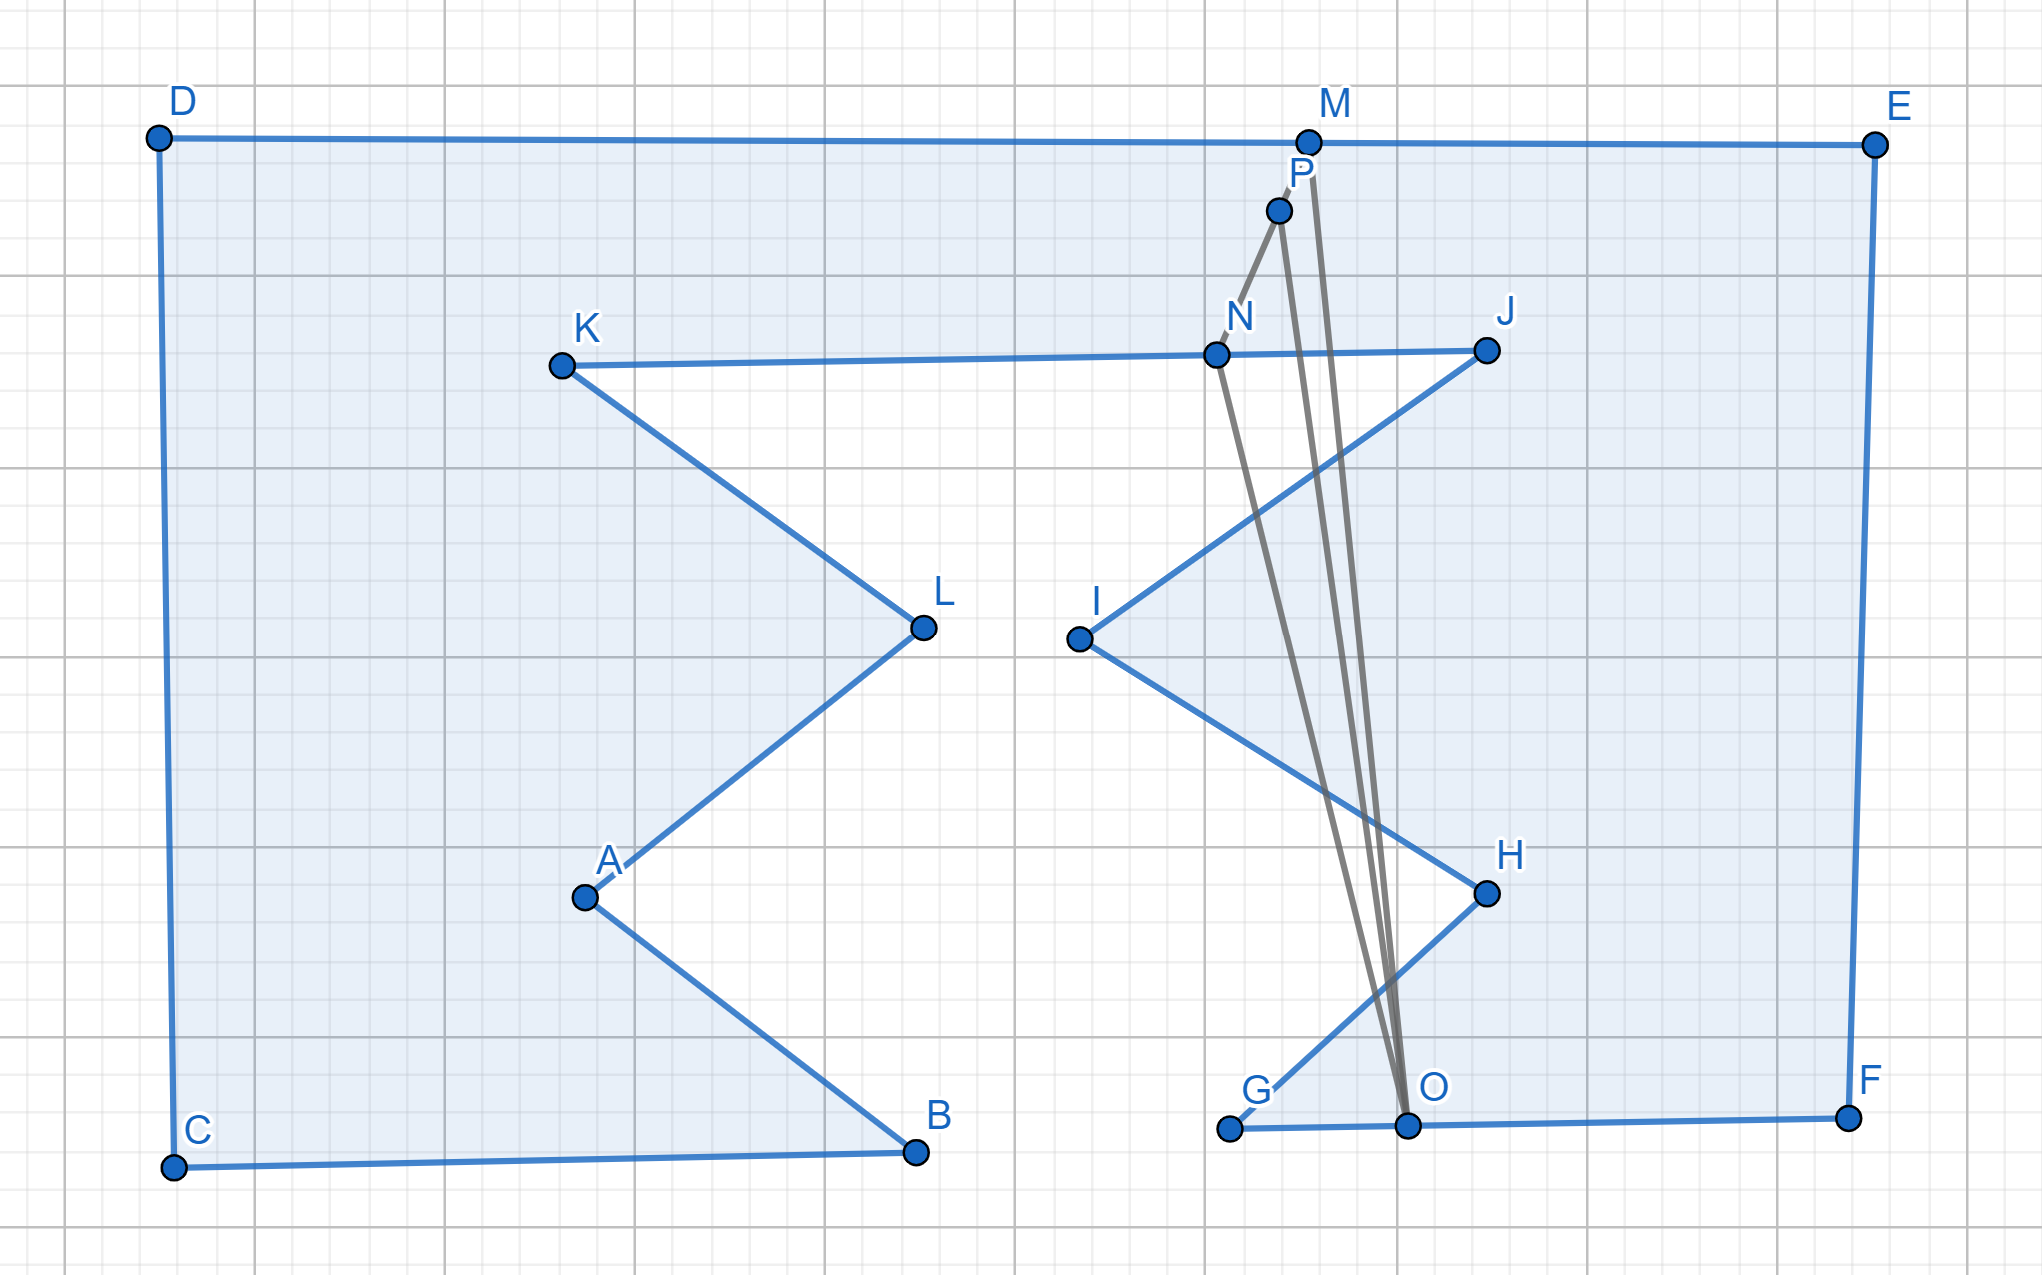
\includegraphics[scale = 0.5]{disconnected.png}


\begin{proof}
Notice that any point in $P$ can be 2-seen the points $L$ and $I$, since any line connecting points in $L$ to points in the reset of $P$ crosses through the boundary at most twice. Similarly, note that any points on the line $NM$ must pass through the boundary of the polygon four times to see the point $O$. Therefore none of the points of $NM$ are in the 2-kernel. Any path connecting $L$ and $I$ must pass through $NM$, and it follows that $L$ and $I$ are not connected by a path within the 2-kernel. Hence the 2-kernel is not connected.
\end{proof}


I think we could talk about $2n$-visibility in general.
The notation and definition of connectedness is 

\begin{proposition}
There exists a polygon whose 4-kernel is disconnected.
\end{proposition}

\begin{proof}
Consider this guy! \\

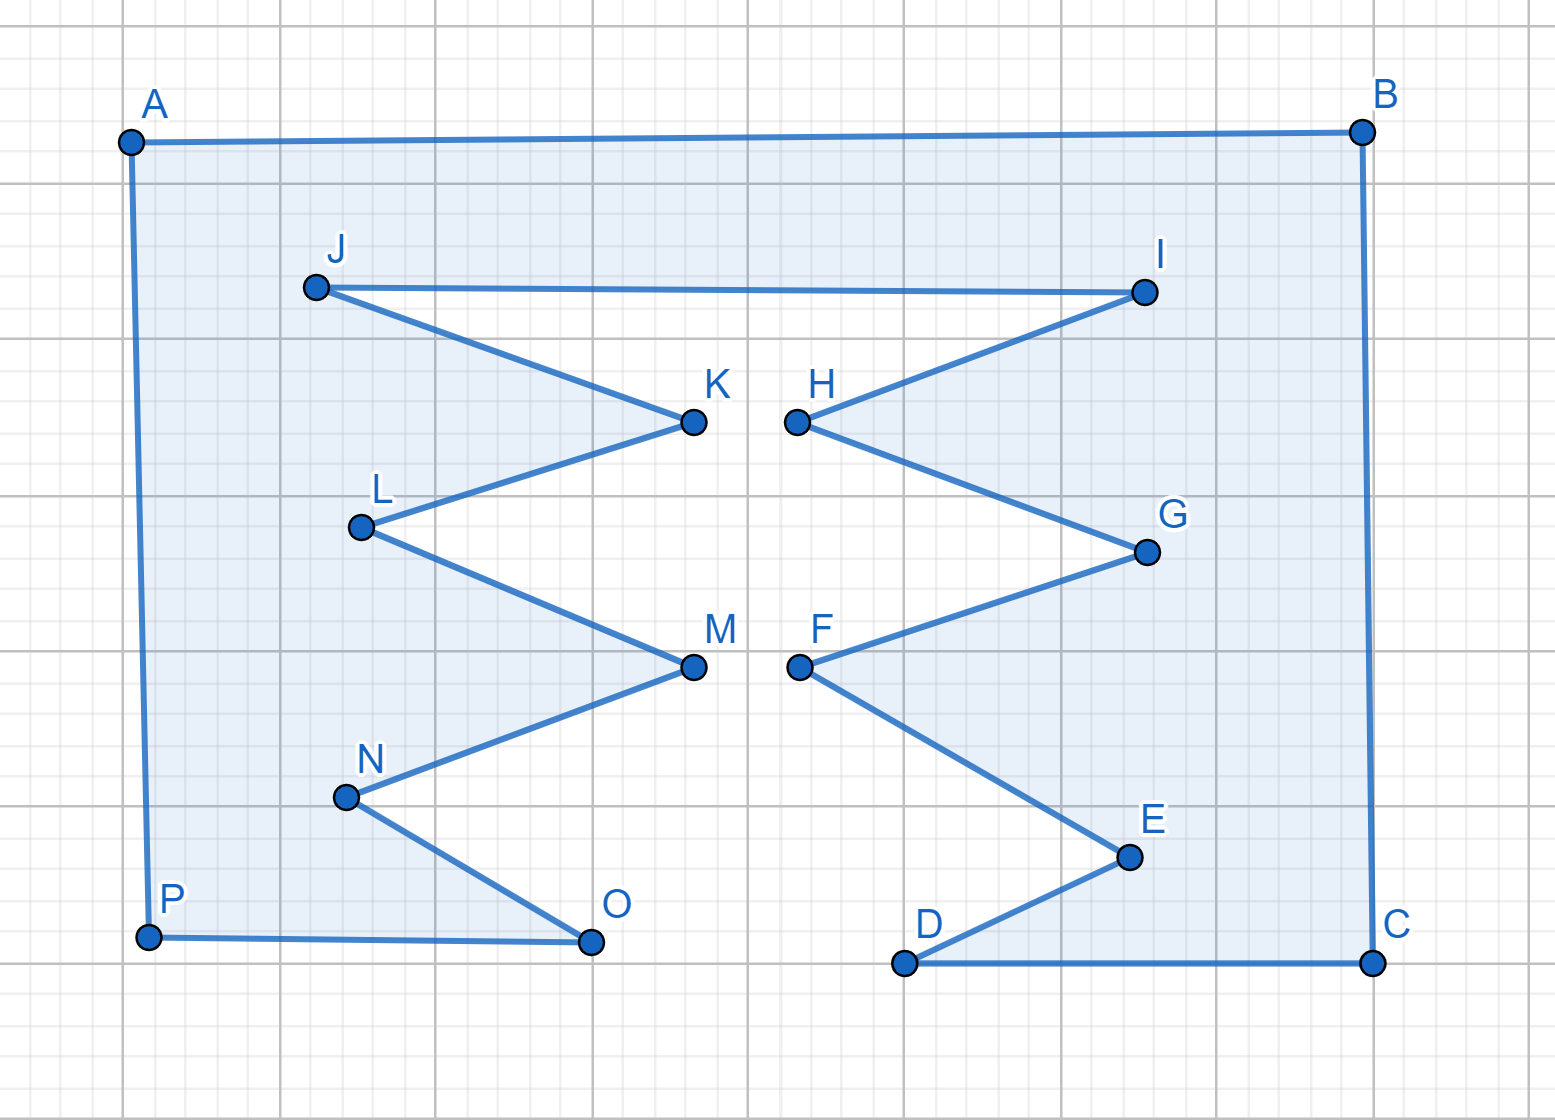
\includegraphics[scale=0.5]{4-kernel.png}
\end{proof}

\begin{proposition}
There exists a polygon $P$ whose 2n-kernel is disconnected, for all $n\in \N$.
\end{proposition}


\begin{definition}
points $x$ and $y$ are 1-connected if they are connected by a single line segment. They are n-connected if they are connected by a polygonal path consisting of $n$ edges. 
\end{definition}

I wonder if it would be possible to extend "visibility" to the number of edges allowed. $1$-connectedness corresponds to visibility, but why not consider $2$-connectedness and above. 

\begin{proposition}
My last conjecture was wrong. There exists a polygon which is not formed in the way I described, and cannot be rotated into the one of them. I have in fact a very powerful class of counterexamples, and a method of constructing them, both of which I shall describe here. Actually, nevermind, here's a picture. 

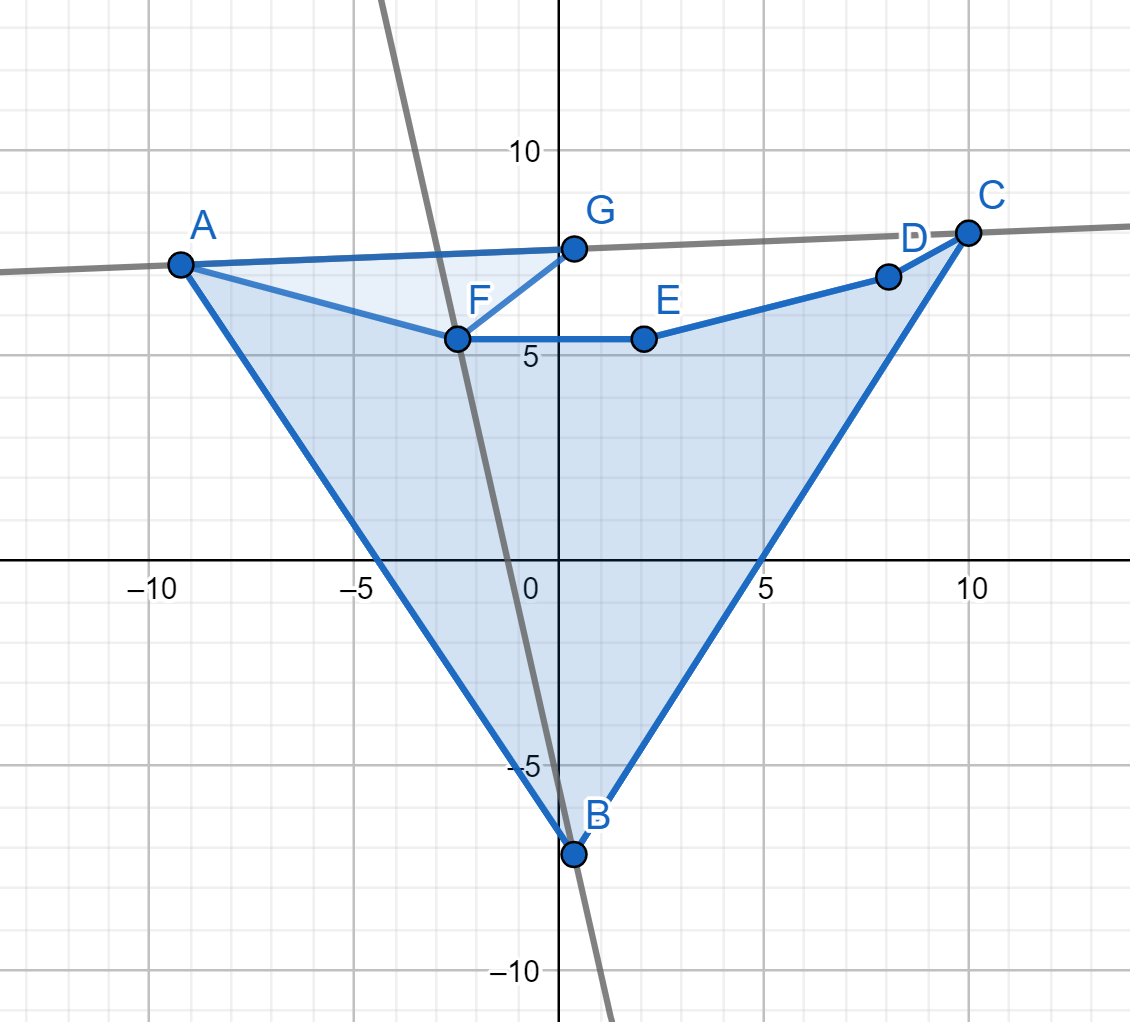
\includegraphics[scale=1]{counterexample.png} 

\end{proposition}

\begin{proof}
Recall my last construction. I shall call these \textbf{convex-uniques}. These convex-uniques can be transformed into a new class of polygons with a unique triangulation, and I have a proof that they cannot be rotated into one of the first class.\\

The same construction is possible, starting with four vertices. Though with four vertices, I can describe a rotation which transforms this construction into one of the last. Consider a quadrilateral $P$ with vertices $v_1, \dots, v_4$, and let $v_4$ be the crux, so that the vertices $v_1,v_2,v_3$ all lie on a curve which is convex up from a line including the point $v_4$ and including all of $v_1,v_2,v_3$ on one side of the line, and where "up" is defined to be the a direction in the side of the line which includes the other points, and where $v_2$ is between $v_1$ and $v_3$. Now draw the lines $v_1v_4$ and $v_2v_4$. 
\end{proof}

\begin{proposition}
It is possible to construct hexagons with $14$, $2$, $4$, $5$, $6$ and $1$ unique triangulations for different hexagons. These can be obtained using a simple type of transformation of the regular hexagon. 
\end{proposition}

\begin{proof}
Consider a regular hexagon $P$. Pick any vertex $v$, and draw rays $r_1,\dots,r_3$, from that vertex to all other vertices on $P$ which are not adjacent. Consider the line which passes through $v$, and which makes equal angles on both sides of $v$. Now draw a curve which concave up with respect to this line (were it to be the x-axis), and which crosses through the adjacent vertices to $v$, and which, between these points, remains entirely within the interior of $P$. This curve intersects the $r_1,\dots, r_3$. Then hexagon with unique triangulation as constructed in my last homework solution, is formed by transforming each of the vertices not adjacent to $v$ to their respective intersections on $r_i$.  The regular hexagon is formed by doing nothing. There are four other options which are distinct up to reflecting the polygon over the middle ray, which won't change the number of triangulations. While this may be convoluted, it's something I've been thinking about while trying to figure out when polygons are "basically the same".\\

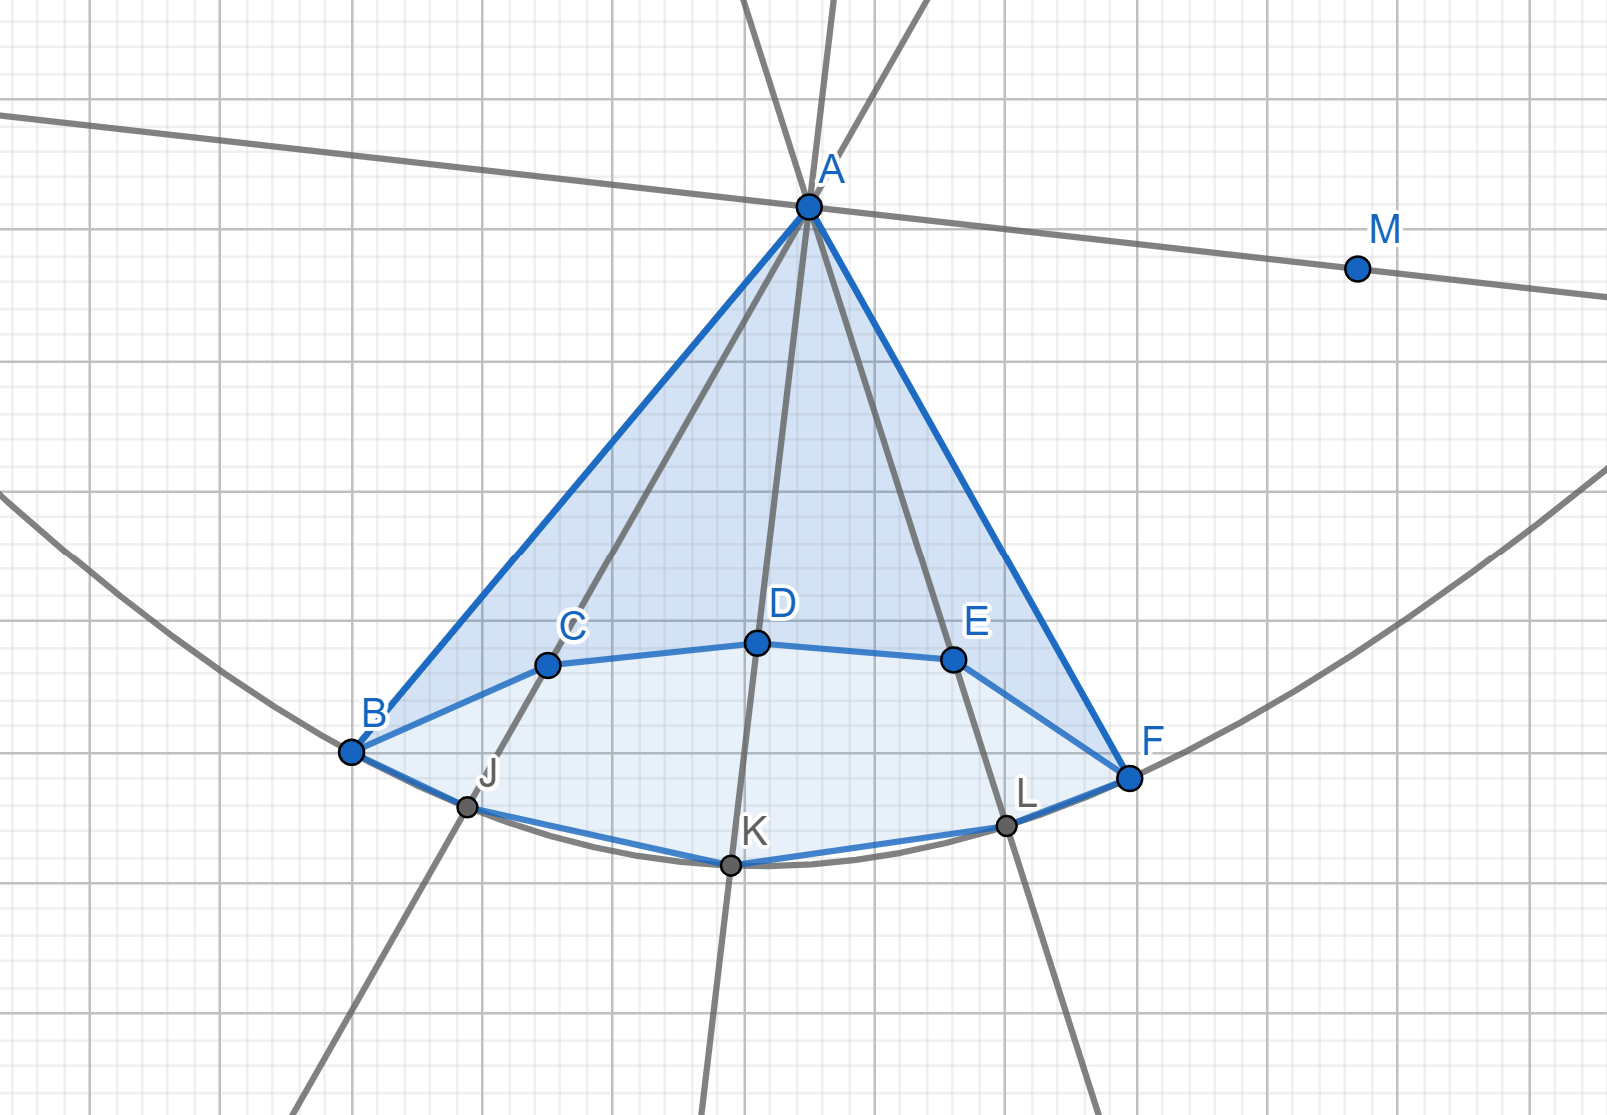
\includegraphics[scale=1]{transformation_2.png} 


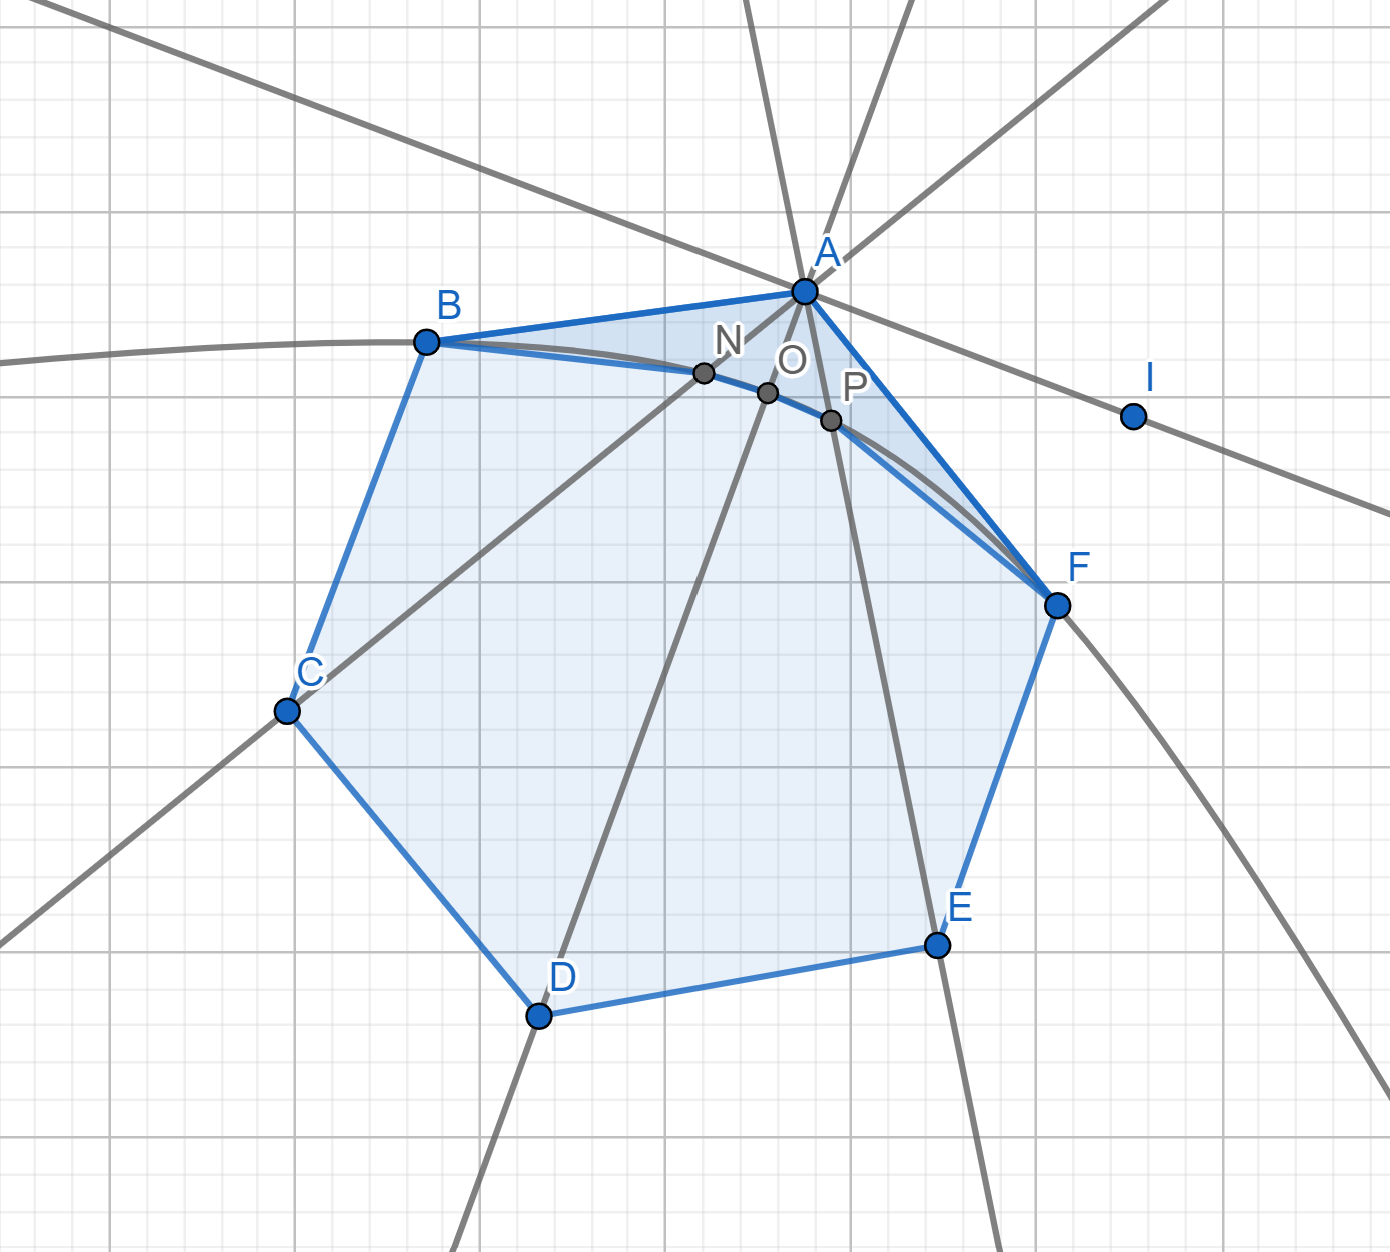
\includegraphics[scale=1]{transformation_1.png} 


This gives us four options: out-out-out (the hexagon), out-in-out, in-in-out, and in-out-in, up to reflection about the middle axis. The 14 and the 1 come from out-out-out, and in-in-in. \\


Suppose we try in-out-out. In this case, we have two diagonals, because we can either draw $v_1v_3$ or not. If we do, we have constructed a "concave-unique". This collapses into one triangulation. If we don't draw the diagonak, we are forced to draw $v_2v$, in which case we have constructed two "concave-uniques". So there are two for this case.\\


Now suppose we try out-in-out. In this case, we are forced to draw $v_3v$, dividing the polygon into two concave quadrilaterals. These have the second catalan number, 2, as their number of triangulations. Hence by the product rule there are total of $4$ triangulations in this case. \\

I had originally been convinced that these were the only possibilities. Ben showed me that this is not the case, and that we can actually get $5$ and $6$ as well. Here's how:


We can also get five different triangulations. Consider the polygon shown below. \\


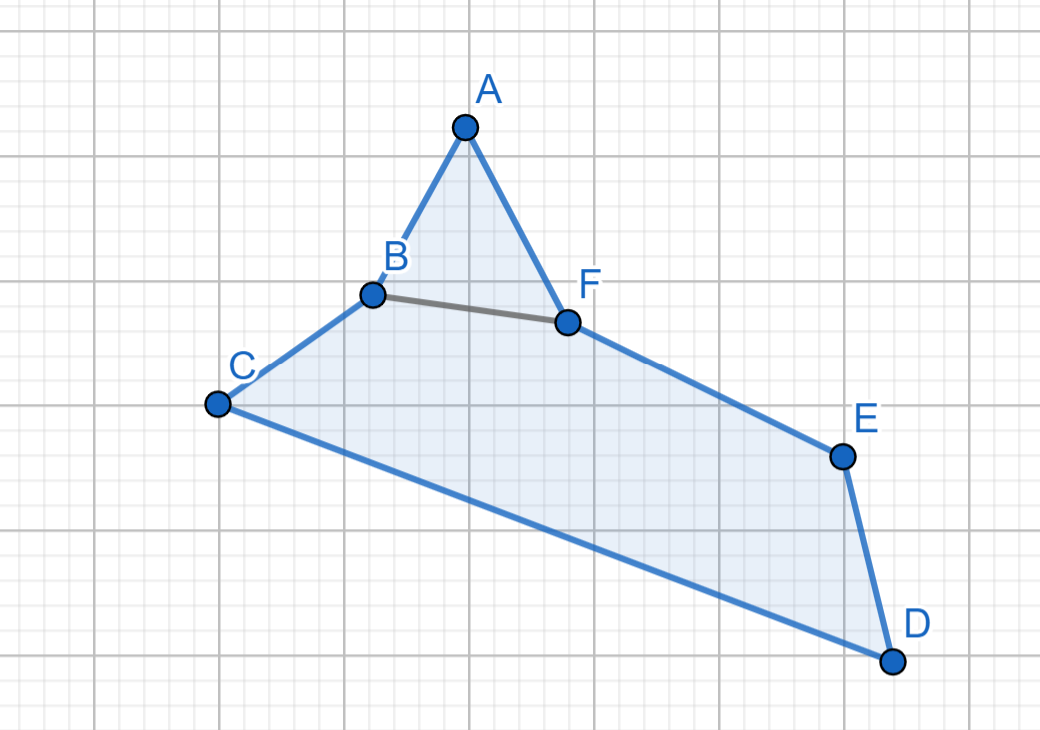
\includegraphics[scale=1]{five.png}\\

Notice that in this case, we are forced to draw the diagonal $BF$. Drawing this, we are left with a convex pentagon, which can be triangulated in five ways. Therefore we have a total of five triangulations for this polygon.\\


We can also get six triangulations. This is how:\\


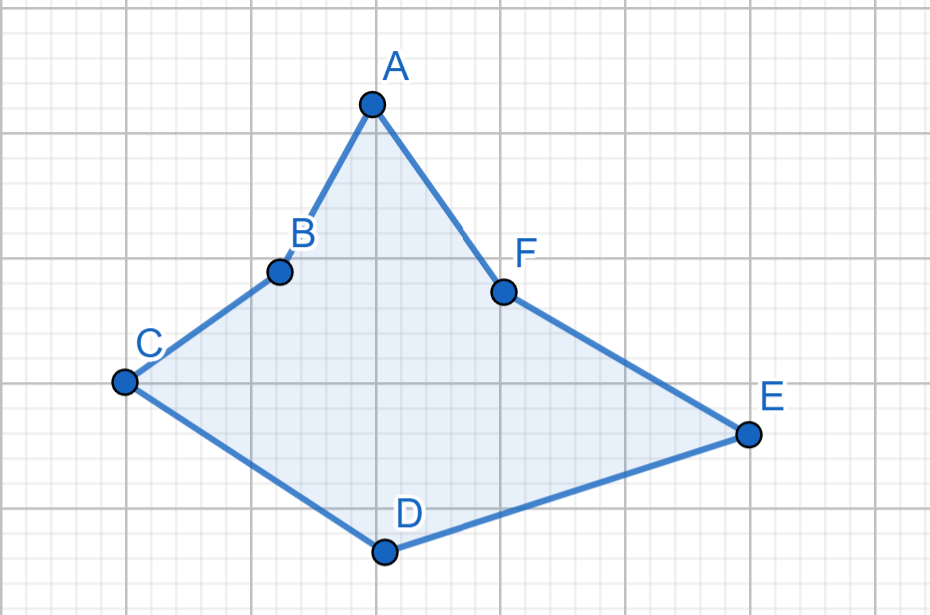
\includegraphics[scale=1]{six.png} \\

In this case, can either draw $BF$ or not. If we do, we have a convex pentagon, and a triangle: which gives us five total triangulations. Now if we don't draw it, we are forced to draw $AD$. In this case, we have two concave uniques, so we must have only one triangulation in this case. In total we have six.

\end{proof}

\begin{proposition} The points $E$, $H$, $K$, $O$, and $S$ form a minimal set of guard points for the polygon below.\\

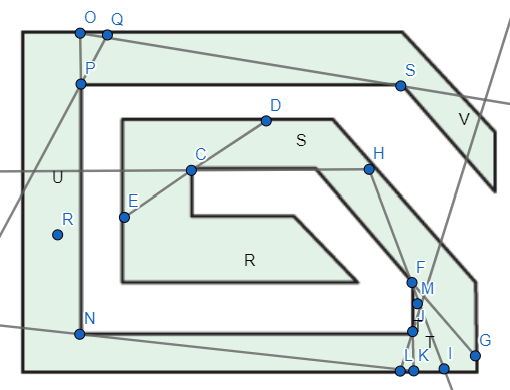
\includegraphics[scale=1]{minimal_2.png}

\end{proposition}

\begin{proof}
While it is easy to find a covering that is small, it is hard to show explicitly that this covering is minimal. I have a sort of "proof" or "method" that I think does the job in this case. First, note that, whatever covering we might use, the region $R$ marked off by $E$ and $C$ must be covered. We must find a point, if we can, that will cover it, and we can't go wrong by covering even more of the polygon in the process. In fact, we must cover $R$ while also covering as much else of the polygon as possible. Notice that any point to the left of $E$ leaves the polygon. Any point to the right of $E$ can see less far beyond $C$. Any point above $E$ must miss part of $R$. Any point below $E$ must also cover less beyond $C$ by making the ray $EC$ "steeper". So then we should chose $E$, for this is the "best we can do" while covering $R$. \\

After placing $E$ as a guard, we note that the region $S$, marked off by the segment $HF$ must also be covered, and indeed it can be covered by one guard. We should try and cover it, while also covering as much as possible while we're at it. If we

Using pretty much the same reasoning, I have placed guards $K$, $O$, and $S$. I would rather not keep on writing this out, for I think what I've written can be "picked up on". I outline the "strategy" or "algorithm" I used here, in hopes that I can generalize it to other polygons.
\begin{enumerate}
\item
\end{enumerate}

\end{proof}

\begin{proposition}
The points $G$ $I$, $D$, $J$ form a minimal set of guards for the polygon shown below.\\

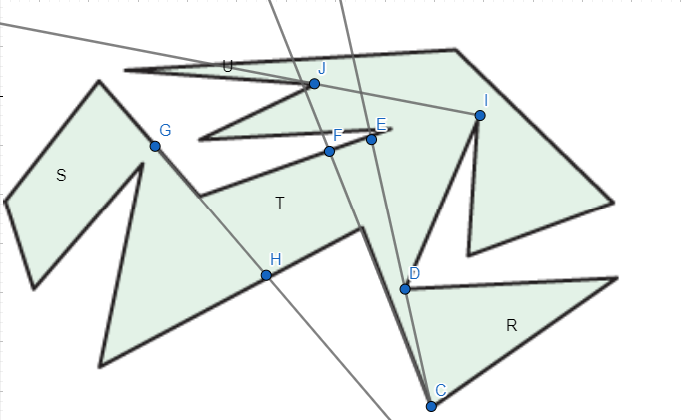
\includegraphics[scale=1]{minimal_1.png}
\end{proposition}

\begin{proof}
Certainly $R$ must be covered, and we should do our best to cover as much of the rest of the polygon as possible, with as few points as possible. Consider the point $D$. Certainly $D$ covers $R$. I'm not sure that this is the best we can do, but it sure feels like it.\\

Now the region $S$ marked off by $G$ and $H$ must also be covered. Consider the point $G$. It covers all of $S$. Moving it won't help all that much more either. Now the region $T$ marked off by the segments $FG$ and $GH$ must also be covered. Consider the point $I$. This is really nice, because it covers pretty much all of the rest of the polygon. Now $U$ marked off by the ray coming from $I$ to $J$ must be covered as well. Welp, $J$ will do, and then we're done. This is minimal because we tried really hard to cover as much as we could the entire way, and trying any harder wouldn't have gotten us any further. I'm really struggling to formalize the process for this one.
\end{proof}

\begin{proposition}
The points $S$, $O$, $P$ form a minimal covering set for the below polygon:\\


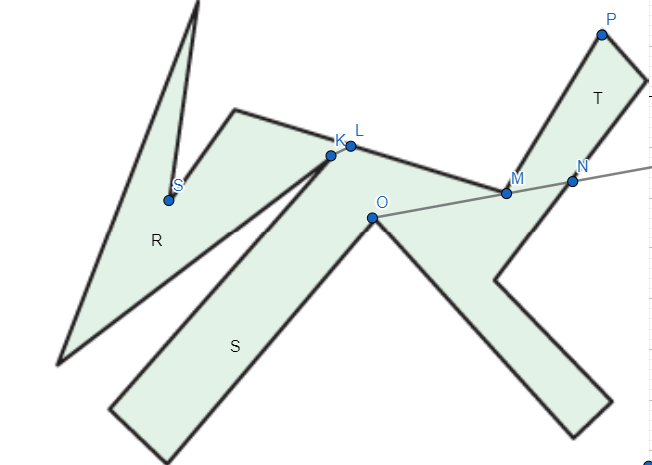
\includegraphics[scale=1]{minimal_3.png}
\end{proposition}

\begin{proof}
We must somehow or another cover the region $R$. Notice that $S$ will do the trick. If we were to move $S$ at all, the line $KL$ would be steeper, covering less of the rest of the polygon, so this really is our optimal choice. We must also cover the reigion $S$. To cover this region, $O$ will do. Anywhere other than $O$ would either not cover $S$, or will miss more of the region $T$ by making the line $MN$ steeper. Finally, we must cover the region $T$. $P$ will do the trick. Because we "tried our best" and made optimal choices the entire way, this must be a minimal covering.
\end{proof}


\end{document}
